\section{湍流非预混火焰}
\subsection{概述}
涉及任何一种燃烧设备,需要考虑的最终要的几个问题:

\begin{enumerate}
    \item 火焰形状和尺寸;
    \item 火焰维持与稳定;
    \item 传热;
    \item 污染排放。
\end{enumerate}

\subsection{射流火焰}
\subsubsection{总论}

\textbf{\textit{初始射流直径}和\textit{燃烧速率}对\textit{火焰尺寸}的影响}:

\begin{figure}[H]
    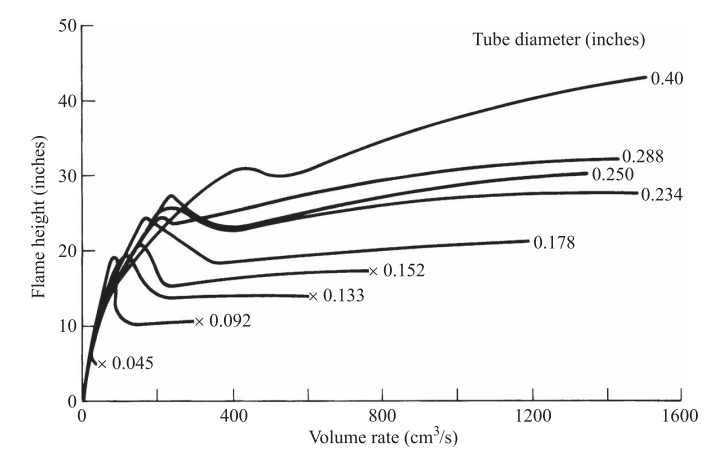
\includegraphics[width=.3\textwidth]{img/q_v_vs_h.png}
\end{figure}

\begin{enumerate}
    \item 流率小、火焰为层流时:火焰高度与初始射流直径无关,只与流率有关;
    \item 当流率增加时,湍流逐渐始影响火焰高度,出现过渡区;
    \item 在过渡区的最后,随着流率的增加,湍流程度不断增加,最后在曲线的极小值点形成比初始层流火焰要短得多的完全湍流火焰;
    \item 当流速进一步增加,火焰高度可能维持不变、也可能不断增加但斜率越来越小,增加的原因是随着燃料流率增加夹带进的空气量和混合速率也会近似成比例增加;
    \item 湍流时火焰高度明显受到初始射流直径的影响。
\end{enumerate}

\begin{multicols}{2}
    \tiny
    \begin{itemize}
        \item \textbf{附着火焰}:在足够低的流速下,火焰根部与燃烧器管子的出口非常接近(只有几个毫米);
        \item \textbf{推举火焰}:当燃料流率增加时,在火焰底部开始形成孔隙,当进一步增大流率时,会形成越来越多的孔隙,直到燃烧器喷口上没有连续的火焰;
        \item \textbf{推举距离}:管子出口与火焰根部之间的距离;
        \item 推举和吹熄。
    \end{itemize}
    
    \textbf{火焰稳定性}:
    \begin{itemize}
        \item 避免推举火焰的产生:可以用火花或者小火焰引燃进行准确的点火并保证火焰位置。但在某些应用条件下,可能需要形成一定的推举量以避免关键的燃烧器部件过热。
        \item 避免接近吹熄极限操作:在接近极限的情况下向很大的炉膛充入空燃混合物是非常危险的,一旦无法及时点燃,混合物在炉内淤积,很可能达到爆炸极限而突然爆炸,造成危险。
    \end{itemize}
\end{multicols}

\subsubsection{简化分析}
\textbf{与冷态射流的对比}
\begin{enumerate}
    \item 在速度和坐标都无量纲化之后,速度场方程时普适的;
    \item 射流扩张角时常数,与射流出口速度和直径无关;
    \item 漩涡年度与流场位置无关,正比于喷嘴出口速度和直径。
\end{enumerate}

当然燃烧后就不能像层流非预混一样和冷态射流那么相似了。浮力的作用使得射流火焰与等温射流之间的相似不再适用这也正好可以解释对于更大直径的喷管,湍流阶段的火焰长度将不恒定。

\textbf{守恒标量回顾}:

守恒标量-混合物分数\(f\)
\begin{eqnarray}
    f &=& \frac{\phi}{(A/F)_\mathrm{stoic}+\phi} \\
    f_s &=& \frac{1}{(A/F)_\mathrm{stoic}+1} \\
    \phi &=& \frac{(A/F)_\mathrm{stoic}}{(A/F)}
\end{eqnarray}

\(f\)的重要特性:
\begin{enumerate}
    \item 火焰边界处的\(f\)值\(f_s\)用来定义火焰边界;
    \item \(f\)只与\(\phi\)有关;
    \item 方程没有源项,\(f\)在整个流场中保持守恒。
\end{enumerate}

\textbf{假设}:还有一些细节可以翻翻书。

\begin{multicols}{2}
    \tiny
    \begin{enumerate}
        \item 稳态、轴对称的时均流场,即燃料由半径为R的圆管射出,在静止、无限大的空气中燃烧。
        \item 与湍流输运相比,动量、组分和能量的分子输运相对不重要。
        \item 湍流动量扩散系数,即旋涡黏度,在整个流场中守恒,且\(\epsilon=0.0285 v_e R\)。通过忽略密度的脉动,将11章提出的恒密度射流的混合长度假设扩展到变密度反应射流。
        \item 忽略所有关于密度脉动的相关项。
        \item 动量、组分和能量的湍流输运都相等:施密特数\(\nu/\mathcal{D}\)、普朗特数\(\nu/\alpha\)和路易斯数\(\alpha/\mathcal{D}\)都相等。
        \item 忽略浮力。
        \item 忽略辐射传热。
        \item 只考虑径向的动量、组分和能量的湍流扩散,忽略轴向的。
        \item 喷嘴出口处燃料射流速度相同,即帽式分布。
        \item 混合物性质由燃料(假想燃料)、氧化剂和产物三种组分决定。
        \item 在采用状态关系式确定平均密度时,忽略混合物分数的脉动。
    \end{enumerate}
\end{multicols}

\textbf{守恒定律的应用}
湍流雷诺数的定义:
\begin{equation}
    Re_T \equiv \frac{v_e R}{\epsilon}
\end{equation}

根据假设10和假设11,温度的状态参数式是\(\overline{f}\)的简单分段线性方程:
\begin{figure}[H]
    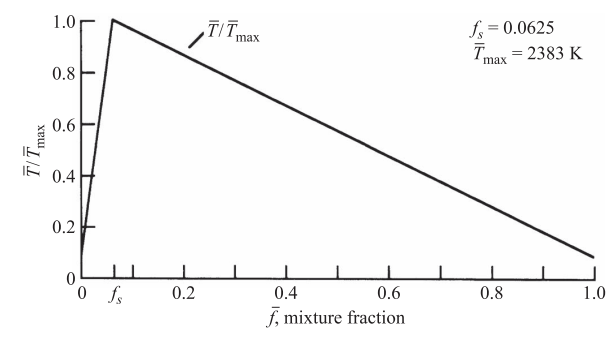
\includegraphics[width=.3\textwidth]{img/f_vs_t.png}
\end{figure}

\textbf{模型解}

\begin{enumerate}
    \item 火焰的高度是喷嘴直径的45倍;
    \item 长宽比(火焰高度和宽度的比值)约11:1,该值比用碳氢射流火焰实验测定的7:1要大一些。
    \item 尽管对湍流射流火焰模型作了大量简化,火焰的总体特征还是能够得到良好的预测,只是精度差些。忽略密度脉动的变化可能对计算准确性影响最大。
\end{enumerate}

\subsubsection{火焰长度}
火焰的可视长度要大于靠温度或浓度测量所得出的长度。

\textbf{影响火焰长度的因素}
\begin{enumerate}
    \item 火焰中射流初始动量与作用在火焰上浮力的比:\(Fr_t\);
    \item 化学当量值\(f_s\);
    \item 射流密度与环境气体密度的比\(\rho_e/\rho_\infty\);
    \item 初始射流直径\(d_j\)。
\end{enumerate}

湍流射流火焰弗劳德数\(Fr_f\)的定义:
\begin{equation}
    Fr_f = \frac{v_e f_s^{3/2}}{{\left(\frac{\rho_e}{\rho_\infty}\right)}^{1/4}{\left[\frac{\Delta T_f}{T_\infty}g d_j\right]}^{1/2}}
\end{equation}
其中\(\Delta T_f = T_f - T_\infty\),表示因燃烧产生的特征温升。
\begin{itemize}
    \item \(Fr_f\)很小,火焰受浮力控制;
    \item \(Fr_f\)很大,初始射流动量决定混合及火焰中的速度场。
\end{itemize}
\textbf{浮力对射流火焰的影响}:
\begin{figure}[H]
    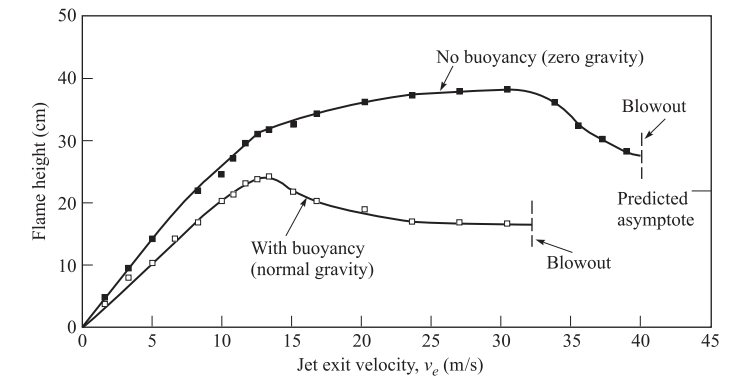
\includegraphics[width=.3\textwidth]{img/buoyancy.png}
\end{figure}
\begin{itemize}
    \item 由于浮力引起的流动,增强了火焰中各成分混合,导致火焰长度比无浮力情况下的长度要短很多;
    \item 如果火焰一直没有吹熄现象发生,随着射流速度的增加,火焰长度最终接近同一渐近值。
\end{itemize}

\textbf{当量值}:\(f_s\)比较小的燃料需要更多的空气才能达到燃烧的化学当量;\(f_s\)越小,火焰越长;丙烷需要的当量空气质量是一氧化碳的6倍,所以丙烷火焰的长度大概是一氧化碳火焰长度的7倍。

\textbf{动量直径}组合了第三和第四个因素的影响:
\begin{equation}
    d_j^* = d_j(\rho_e/\rho_\infty)^{0.5}
\end{equation}

\textbf{关联性}
\begin{figure}[H]
    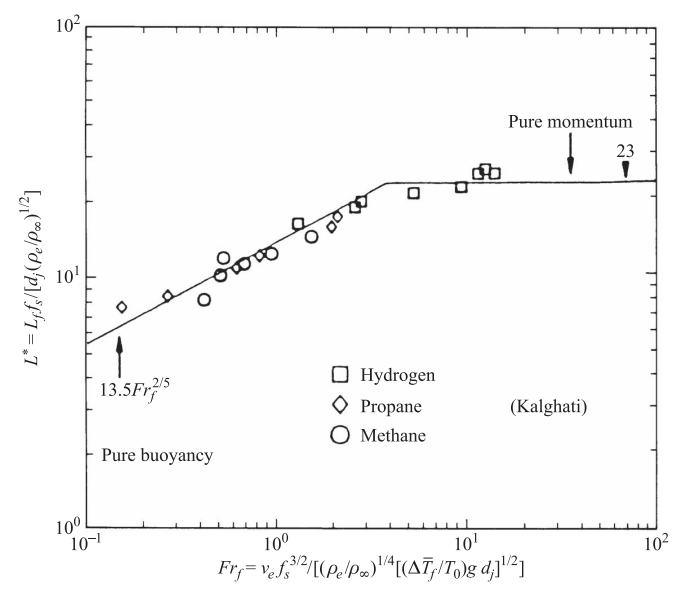
\includegraphics[width=.3\textwidth]{img/fr.png}
\end{figure}
无量纲火焰长度:
\begin{equation}
    L^* = \frac{L_f f_s}{d_j (\rho_e/\rho_\infty)^{0.5}}
\end{equation}

\begin{enumerate}
    \item 浮力控制:
    \begin{equation}
        L^* = \frac{13.5 Fr_f^{0.4}}{(1+0.07 Fr_f^2)^{0.2}}, \quad Fr_f < 5.0
    \end{equation}
    \item 动量控制:
    \begin{equation}
        L^* = 23, \quad Fr_f\ge 5.0
    \end{equation}
\end{enumerate}

\subsubsection{火焰辐射}
\textbf{辐射分数}\(\chi_R\):
\begin{equation}
    \chi_R = \frac{\dot{Q}_\mathrm{rad}}{\dot{m}_\mathrm{F}\Delta h_c}
\end{equation}
其中\(\dot{m}_F\)是供给燃料的质量流率;\(\Delta h_c\)是燃料的热值

\begin{enumerate}
    \item 燃料的辐射分数与发烟点相对应;
    \item 辐射分数的大小由火焰尺寸和释热率决定:当固定燃烧速率而减小火焰尺寸,或固定火焰尺寸而增大燃烧速率时,都会使辐射分数 减小。    
\end{enumerate}

\subsubsection{推举和吹熄}

有三种理论可以解释推举火焰:
\begin{enumerate}
    \item 层流火焰速度最大处的局部气流速度恰好与湍流预混火焰的燃烧速度相等:\(\overline{v}(S_{L,\max})=S_T\);
    \item 流场局部的应变速率超过了层流扩散火焰面的临界熄火应变速率:\(\epsilon>\epsilon_{crit}\);
    \item 大尺度流场结构中高温产物与未燃混合物的有效返混时间小于点火的临界化学反应时间:\(\tau_\mathrm{local-mixing}<\tau_\mathrm{chem,crit}\)。
\end{enumerate}

\begin{enumerate}
    \item 推举高度与烧嘴直径之间没有多少相关性;
    \item 层流火焰速度越大,推举高度h曲线增加的斜率越大。
\end{enumerate}

\textbf{火焰吹熄的原因}:当流速增加时,推举高度不断上升。火焰根部的流速和湍流燃烧速度都随推举距离的增加而减小。在某个临界点之后,湍流燃烧速度的减小速率>局部流速的减小速率(最大层流燃烧速度处),再也找不到可以平衡的点,两者差距越来越大,发生吹熄。


有关系式可以计算射流火焰吹熄速度,具体可以看416页。当燃料固定,吹熄速度将随射流直径的增加而增加。这也就是为什么油井熄火十分困难的原因(通常油井直径比较大)。

\subsection{其他结构下的非预混火焰}
应用旋流主要有两个原因:第一,当旋流足够大时,可以产生回流区来稳定火焰;第二,旋流的程度还可以控制火焰的长度。

旋流数\(S\)的定义:\(S=M/(I r_0)\),其中\(M\)是切向动量矩,\(I\)是轴向动量,\(r_0\)为特征尺寸。当\(S\ge 0.6\)时为强旋流。

旋流火焰的作用:
\begin{enumerate}
    \item 稳定火焰:
    \item 控制火焰长度:旋流大大加强了空气与燃料的混合。
\end{enumerate}